\documentclass{article}
\usepackage{float}

% Language setting
% Replace `english' with e.g. `spanish' to change the document language
\usepackage[english]{babel}

% Set page size and margins
% Replace `letterpaper' with`a4paper' for UK/EU standard size
\usepackage[letterpaper, top=1.5cm, bottom = 1.5cm, left = 1.5cm, right = 1.5cm, marginparwidth=1.75cm]{geometry}

% Useful packages
\usepackage{amsmath}
\usepackage{graphicx}
\usepackage[colorlinks=true, allcolors=blue]{hyperref}

\title{Exploring the relationship between climate attitudes and extreme weather events - S\&DS 625 Final Project}
\author{Megan Ayers}


\begin{document}
\maketitle

\section{Introduction}
\subsection{Contextualizing and motivating}
Climate change and environmental degradation is one of the most existential
crises of our time, if not the most existential. Unfortunately, many
Americans do not agree with this statement and/or do not fully comprehend the
implications of our global future if we do not address the causes of
climate change. Without recognition of the seriousness of climate change,
harmful consumer habits perpetuate, eco-friendly policies falter due to lack
of support, and the industries and corporations that negatively impact the
environment are not held accountable nor pressured to abandon the status-quo.
Climate communication is a field that works with these issues, and in
particular, with how to educate and persuade individuals about climate
change and the necessity of acting to reduce it. The hope is that
the more people there are that recognize climate change as a serious threat,
the more likely we are to have politicians and corporations that are
pressured to use their positions of power to enact positive change when it
comes to the environment. 

This contextualizes the goal for this final project - to better understand
some aspects of climate change beliefs at the county-level. If we don't 
understand the beliefs that people currently have about climate change,
and what factors might influence those beliefs, then we will be less
effective at trying to persuade those people than if we can be understanding
and empathetic at the same time as being convincing. In particular, this
report investigates how local extreme weather events relate to county-level
climate change beliefs. Perhaps personally experiencing one of
the widely broadcasted affects of climate change - increased extreme weather
events such as drought, hurricanes, wildfires, winter storms, etc - would
cause a person to take climate change more seriously, compared to someone
who just hears about these things happening on the news. However, there are
other cultural and demographic factors that are expected to have an effect
on climate change opinions that also need to be controlled for, such as
political leanings and age. To understand these factors and to attempt to quantify the relationship between experiencing extreme weather and climate change beliefs, a few different approaches were used: exploratory data analysis and manual clustering to look for high level and heterogeneous relationships, a matching procedure to directly compare similar counties that differed on their experience of extreme weather, and linear regression to try to understand how all covariates, including extreme weather experience, correlate with climate change opinions. 


\subsection{Data sources}
To explore the relationship between extreme weather events and climate
change opinion with consideration given to the additional impact of
political leanings and demographics on climate change beliefs, the analysis
draws on information from multiple data sources. 

Data collected and processed by the Yale Program on Climate Change
Communication is used to understand climate change belief (the response
variable of this analysis). This data consists of US
county-level estimates of climate change beliefs, i.e. x\% of the population
in New Haven County believes that climate change is happening. These
estimates are calculated from a large-scale nation-wide survey ($n > 25,000$)
conducted in spring of 2020, and were "derived from a statistical model using
multilevel regression with post-stratification (MRP)". Though using
individual-level data could be more convincing for arguing existence of a
relationship between extreme weather event experiences and climate change
beliefs (the unit "county" does not itself have a climate change belief),
actually obtaining the supplementary data at this level was not feasible for
this project due to data privacy issues. 

Supplementary demographic data at the county level was collected from the Census
Bureau's ACS 2019 estimates using the R package `tidycensus`. To understand
the political leaning of each county, 2020 general election results were obtained
at the county level. These came from a data set containing general election
results from 2000-2020 maintained by the MIT Election Data and Science Lab
and accessed via the Harvard Dataverse. 

Identifying counties that experienced an extreme weather event around the
time of the climate opinion survey is not cut-and-dried. How should one
define "extreme weather"? There may be multiple reasonable responses
to this question, but this report defines "extreme weather" as
weather events that were declared disasters by FEMA
(Federal Emergency Management Agency). Records of these events from 1953 to
2021 are recorded in the online OpenFEMA Data Sets at the state and county level.
FEMA disasters were chosen as the indicator of extreme weather because
they signal a disaster beyond what state governments typically expect and are
prepared to handle. This accounts for the fact that independently of climate
change, some parts of the country naturally experience - and are used to
experiencing - more severe weather than others.


\section{Data Preparation}

Merging these data sources required cleaning and quality
assurance checks of each individual source.

\subsection{Climate change opinion survey data}
Because the providers of the climate change opinion survey already processed
the individual responses into county-level estimates, this data is very clean
to begin with. Data is available for every county reported on by the Census
in 2020, there are no duplicate rows, and the response variable `happening`
(indicating the proportion of county population that believes climate change
is happening) is relatively Normal in distribution (a QQ-plot of this is included in the appendix for reference). Note that the original
survey file contains data for many different climate-related questions asked
in the survey, but this analysis focuses only on the high level
question of existence of climate change.

\subsection{Election data}
This data set required a little more work to clean up. Data was reported for
one county that was not recognized as a county by the Census, and was dropped. For
some reason, San Joaquin County CA had missing data, which was found 
manually from the county website and replaced. Votes were sometimes
recorded by the mode in which they were received (ex. "Early Vote", 
"Absentee", "Election Day" etc.) and sometimes in total, so aggregation to 
the total county level had to be standardized between counties. All differences in county names between this source and the 
Census Bureau (which was regarded as ground truth for standardizing all sources
to use FIPS codes for future merging) could be rectified except for voting districts in Alaska.
I was unable to find a way to map voting districts to Census-reported
counties, so I dropped Alaska from the analysis. Although the other data
sources do have information on Alaska, political leaning was clearly such a
strong indicator of climate change belief that it seems preferable to
drop it entirely from the analysis rather than introduce missing values for
political leaning.
Figure 1 shows the geographic distribution of the county-level 2020 election
results, while also indicating whether that county has above or below average
belief in climate change (compared to the political group average, not the
overall average).
Later in the analysis, four counties were found to have had over 100\% of their population reported as having allegedly voted in the 2020 general election. The county population numbers from the Census were verified, which casts the election data for these counties into doubt. Because political leaning was found to be such a strong indicator of climate change opinion, and because none of these counties were considered to have experienced extreme weather as defined later in this section, these four counties were dropped from the analysis.

\subsection{Census demographic data}
The ACS 2019 estimates obtained through the Census were very clean and
required almost no cleaning aside from reshaping the data and renaming one
county to be consistent with a recent name change. The analysis begins with  
information about the gender, race, and ethnicity breakdowns of each county,
along with the median income and age of each county. Population
proportions are calculated for use in the analysis instead of the raw total counts.

\subsection{FEMA weather data}
Given the choice of the FEMA data set, there remains a tension between the
ideas that experiencing multiple events over a longer time scale would have
a larger impact on people's mindsets, but also that it is harder to safely
assume that the same individuals are remaining in the same county over a
longer time scale. In an attempt to balance these competing interests,
counties are flagged as "affected by extreme weather" if they experienced
a FEMA declared event in 2019 (the closest data to when the climate opinion
survey was collected), and also experienced at least 2 FEMA declared events
between 2015-2018. This second requirement is an attempt to capture counties
where extreme weather is more likely to be seen as recurrent rather than a
fluke. 511 (a little over 16\%) US counties meet this requirement. Note that
the original data sets include FEMA disasters that are non-weather related,
such as earthquakes, biological disasters, chemical disasters, terrorist
disasters, etc. This analysis considers hurricanes, floods, severe storms,
fires, snow, tornados, severe ice storms, coastal storms, typhoons, and
droughts. Figure 2 displays all FEMA declared weather disasters from 2015-2019,
as well as highlighting the counties which meet the requirements outlined above
to be considered as "affected by severe weather" in the analysis.

\begin{figure}[H]
\centering
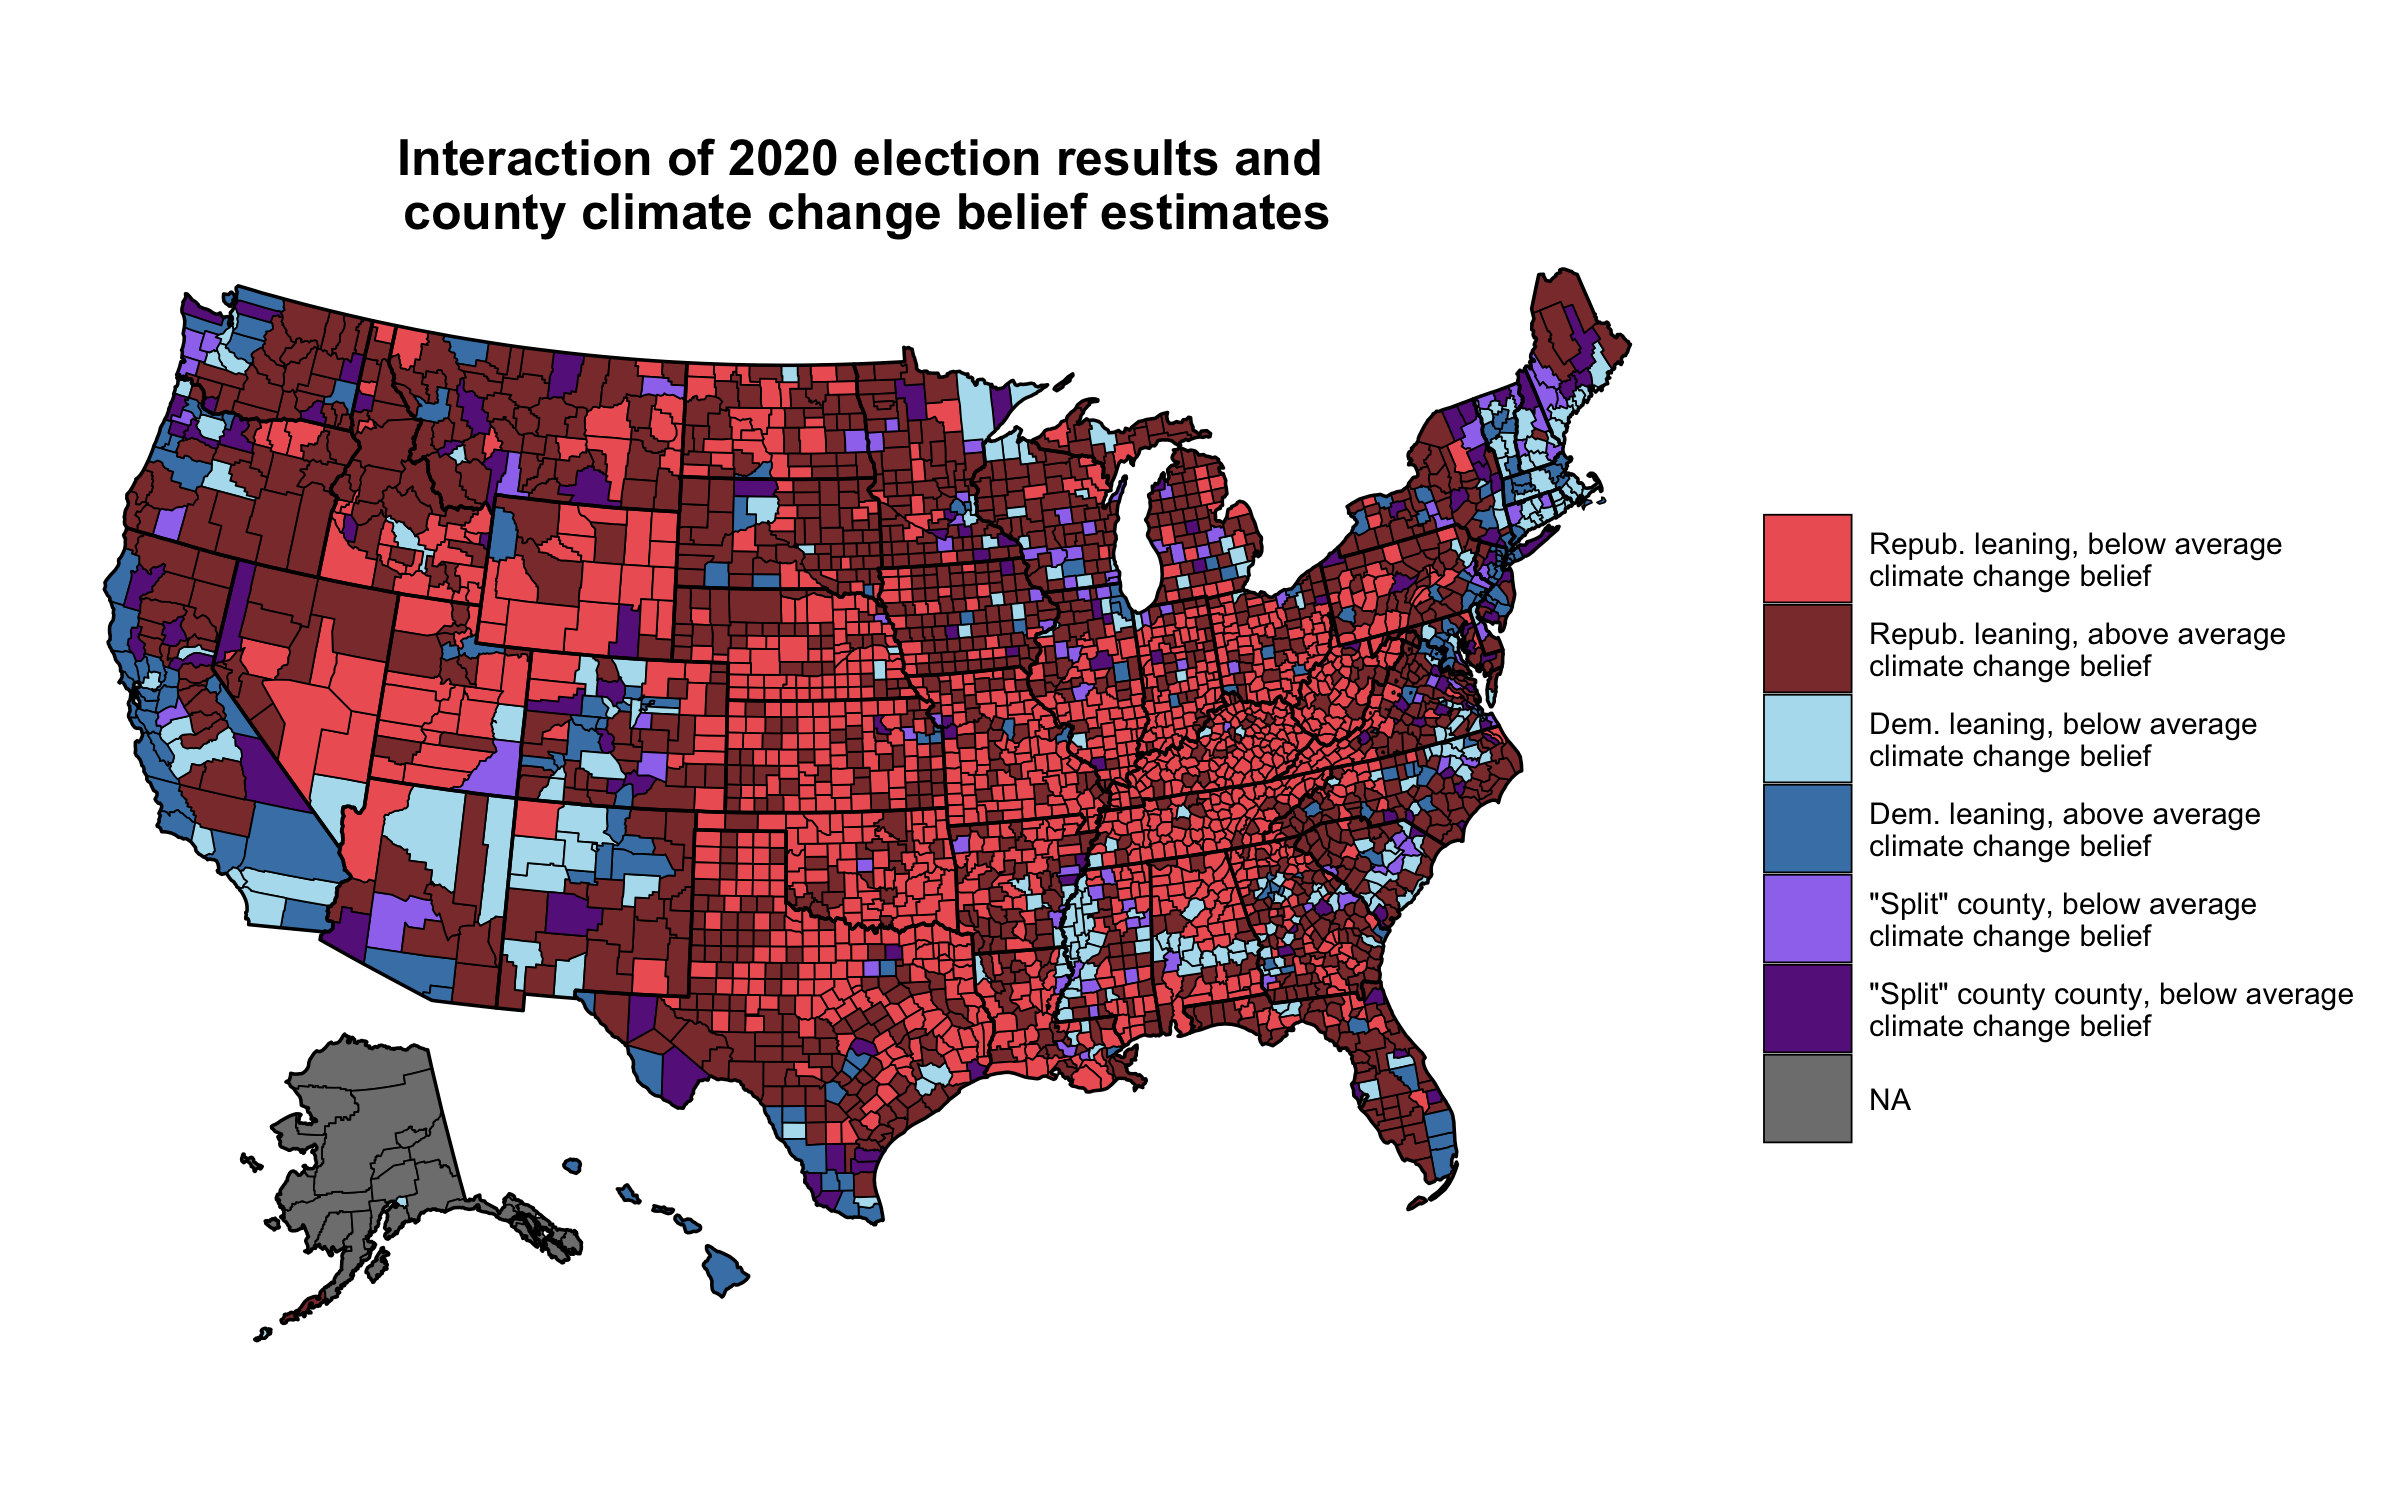
\includegraphics[scale=0.225]{images/election_climate_beliefs_map_in_group_comp.png}
\caption{This figure shows the 2020 presidential election results at the county level while also showing whether these counties have climate change belief above/below average compared to their political group. "Split" counties refers to counties where neither Democrats nor Republicans won more than 52.5\% of the vote.}
\end{figure}


\begin{figure}[H]
\centering
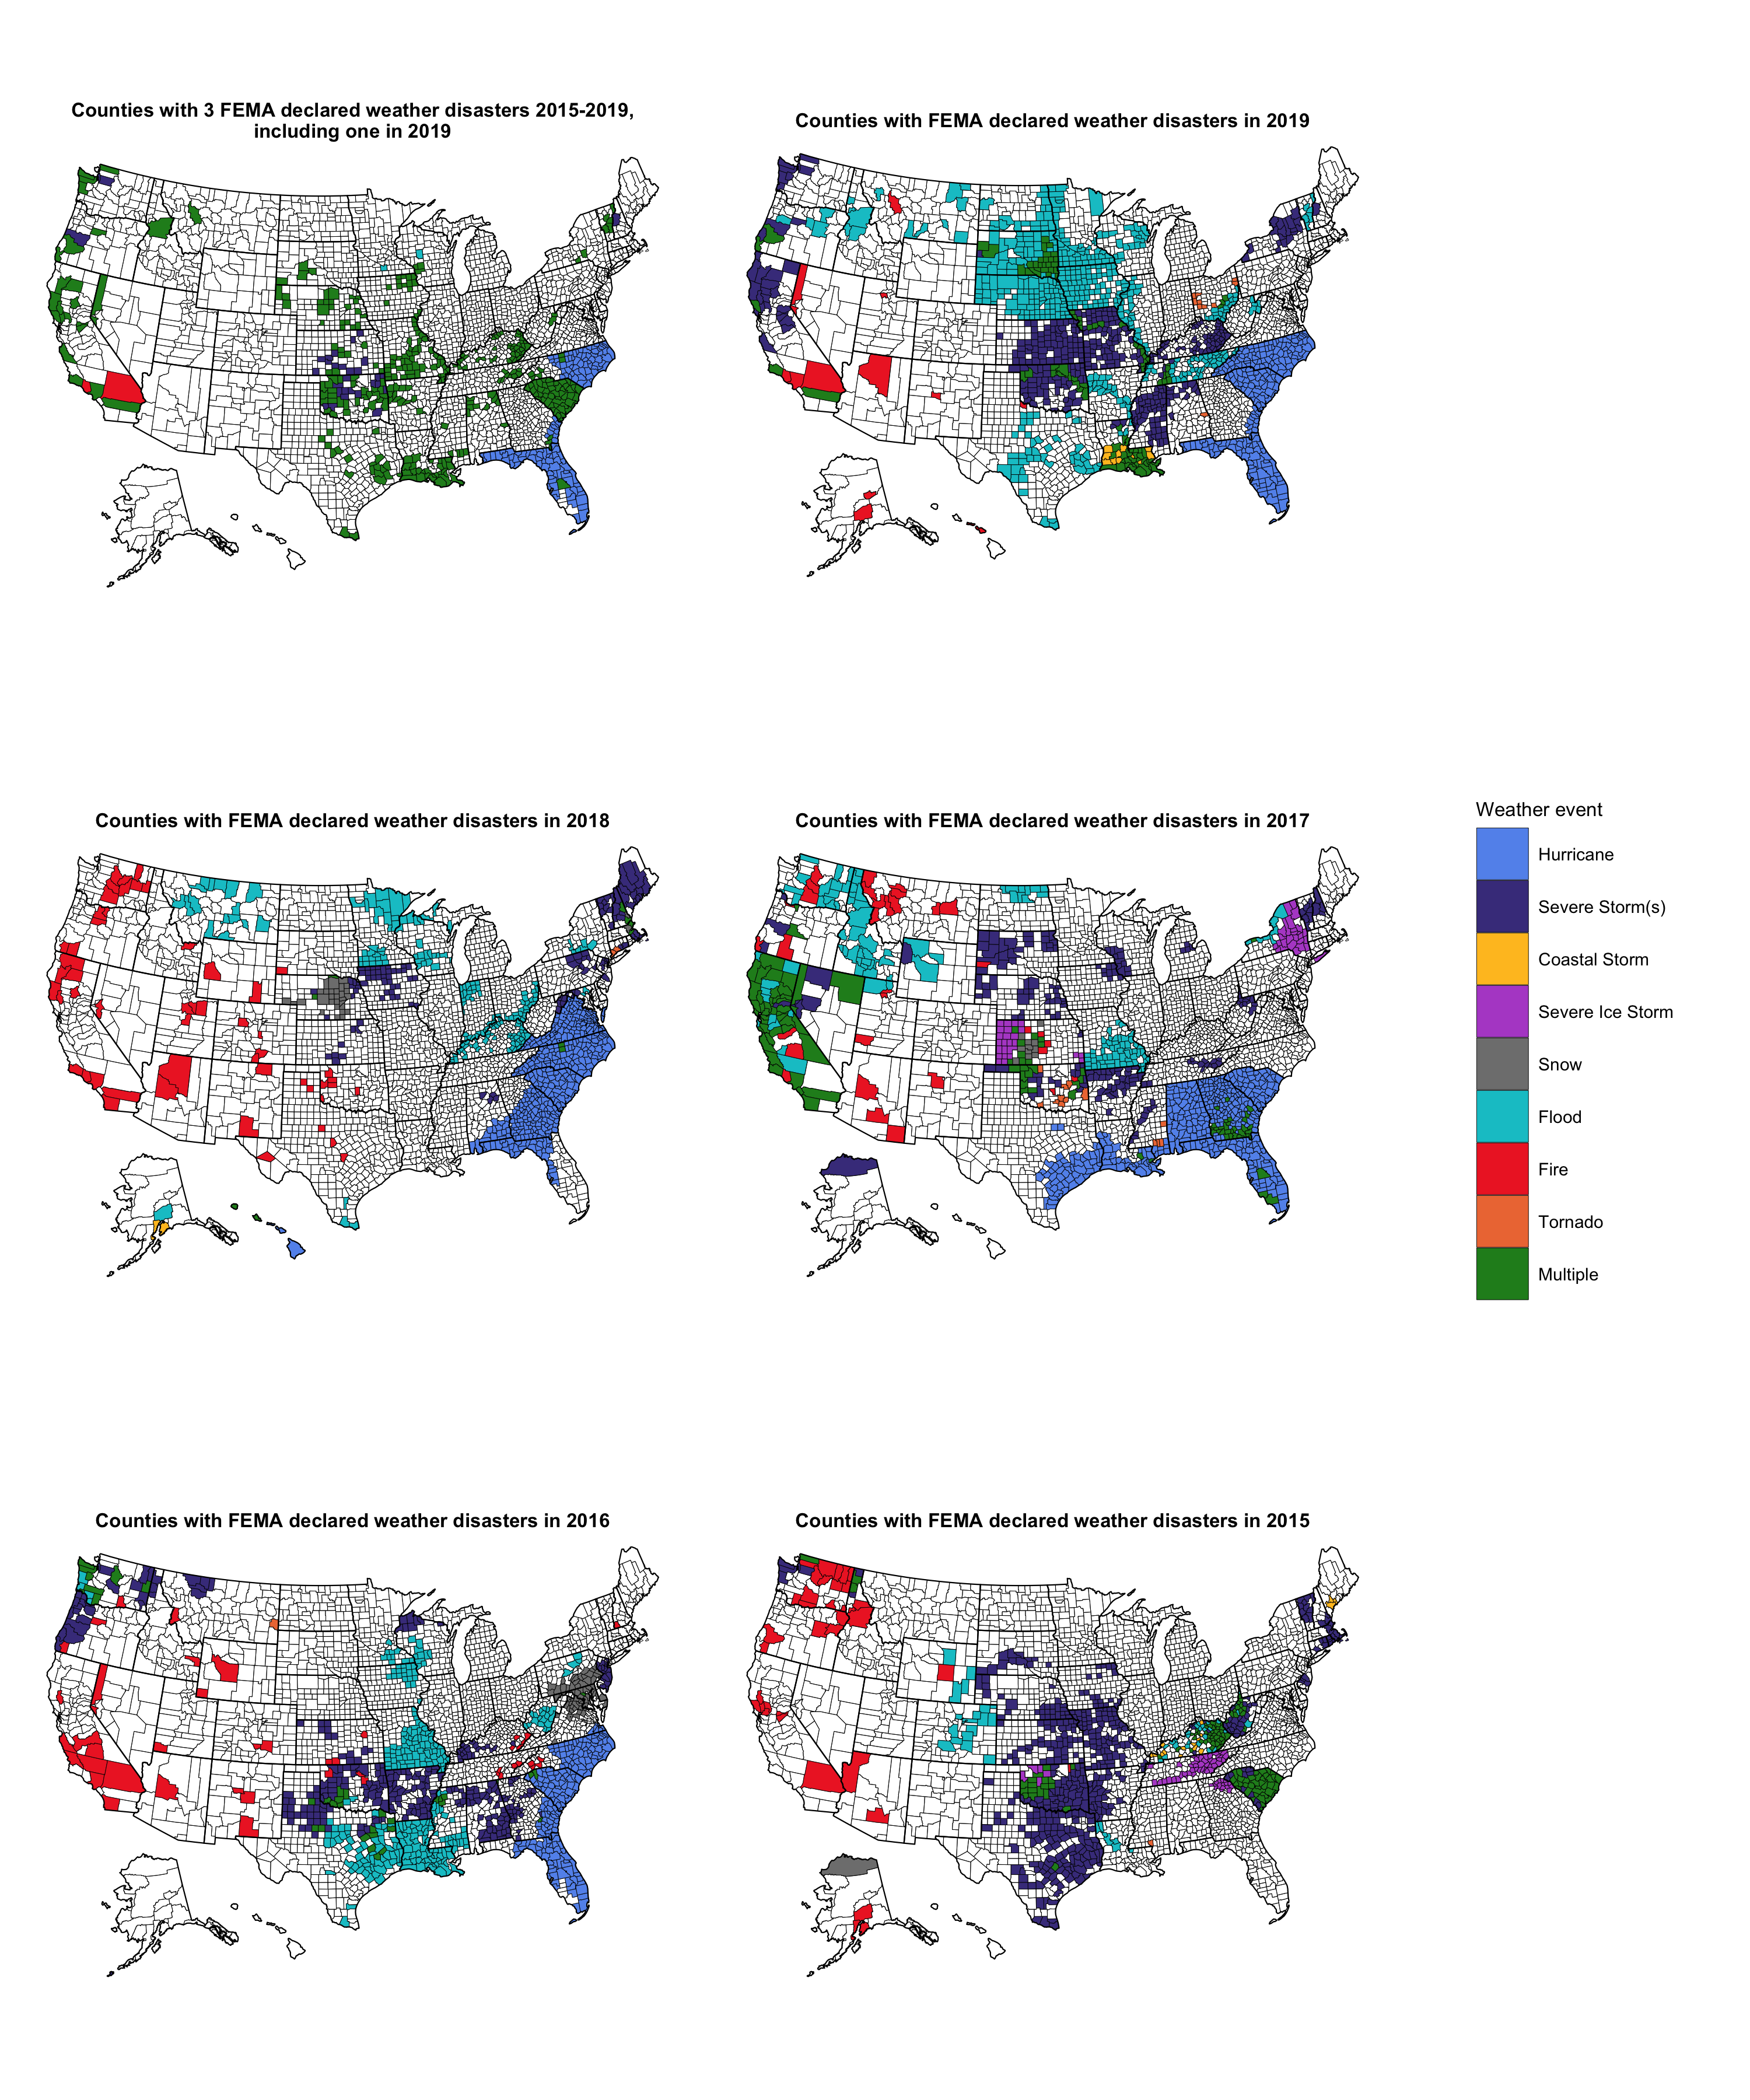
\includegraphics[scale=0.175]{images/fema_events_maps_combined.png}
\caption{Upper left: counties with FEMA declared disasters that are flagged as "affected by severe weather" in this analysis. The rest of the plots show all FEMA declared weather disasters from 2015-2019. Larger plots can be found in code directory.}
\end{figure}

\begin{figure}[H]
\centering
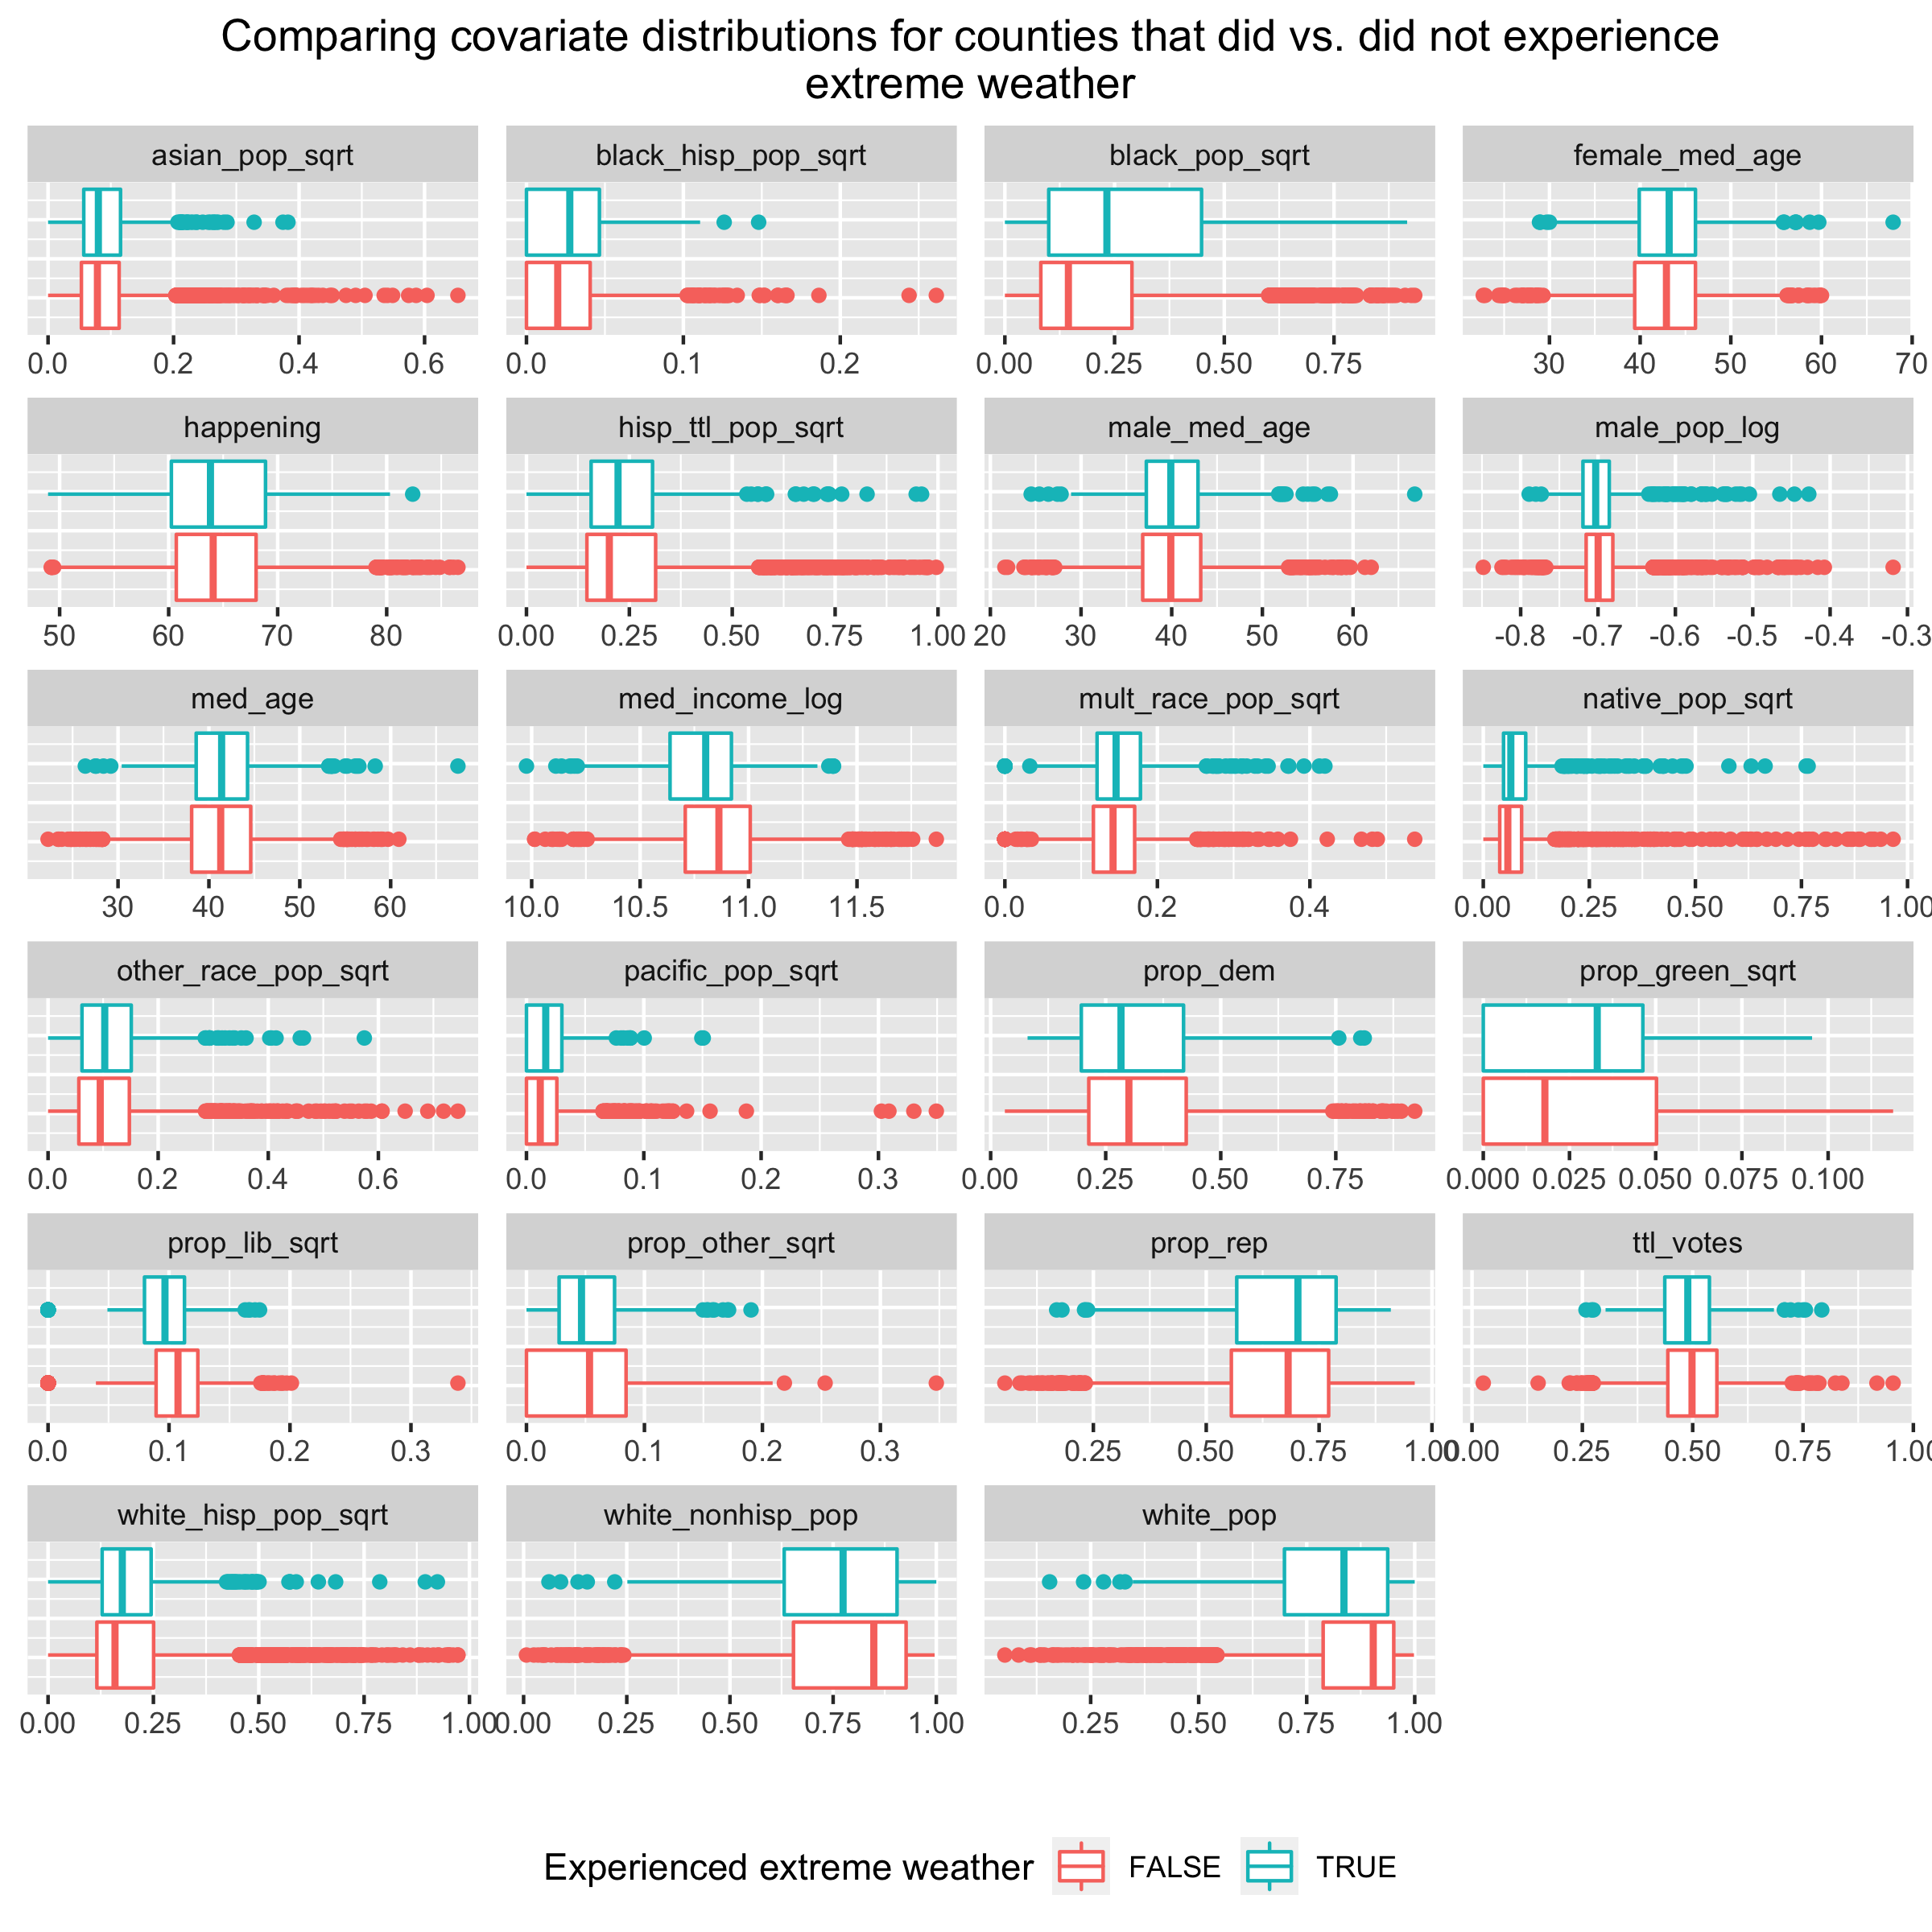
\includegraphics[scale=0.2]{images/covariate_dist_comp.png}
\caption{A boxplot is shown for every continuous covariate collected for this analysis, as well as the response `happening', with the two colors representing counties that did/did not experience extreme weather. Variables that have been transformed have titles ending in sqrt or log.}
\label{covariate_comp}
\end{figure}

\section{Analysis}

\subsection{Exploratory Data Analysis and Covariate Selection}
First, to understand if and how counties that experienced extreme weather differed from those that didn't, some exploratory data analysis was performed. 511 counties met the extreme weather conditions outlined above, leaving 2600 counties as what may informally be referred to as the control group. Between these two groups, the distribution of all collected covariates was compared, as is shown in Figure \ref{covariate_comp}. We can see that there is relatively close agreement in distribution between the groups across covariates. This is not very surprising - the 511 counties that did experience extreme weather are scattered across diverse regions of the country in such a way that it seems reasonable for them to constitute a fairly representative sample of the larger group of counties. 

Next, using all counties, the covariates were compared to `happening' (the proportion of each county estimated to believe that climate change is happening) to observe any visually obvious relationships between the variables and the response. Because an ultimate goal of the analysis was to use linear regression, and to use Lasso as a method for variable selection, variables were transformed using the square root or logarithm transformation if needed to enforce more linear relationships. The square root transformation was applied to those variables that had many zero values in the data, such as proportions of certain race or ethnicity groups in county populations. These plots in their transformed forms can be viewed in Figure 4.

\begin{figure}[H]
\centering
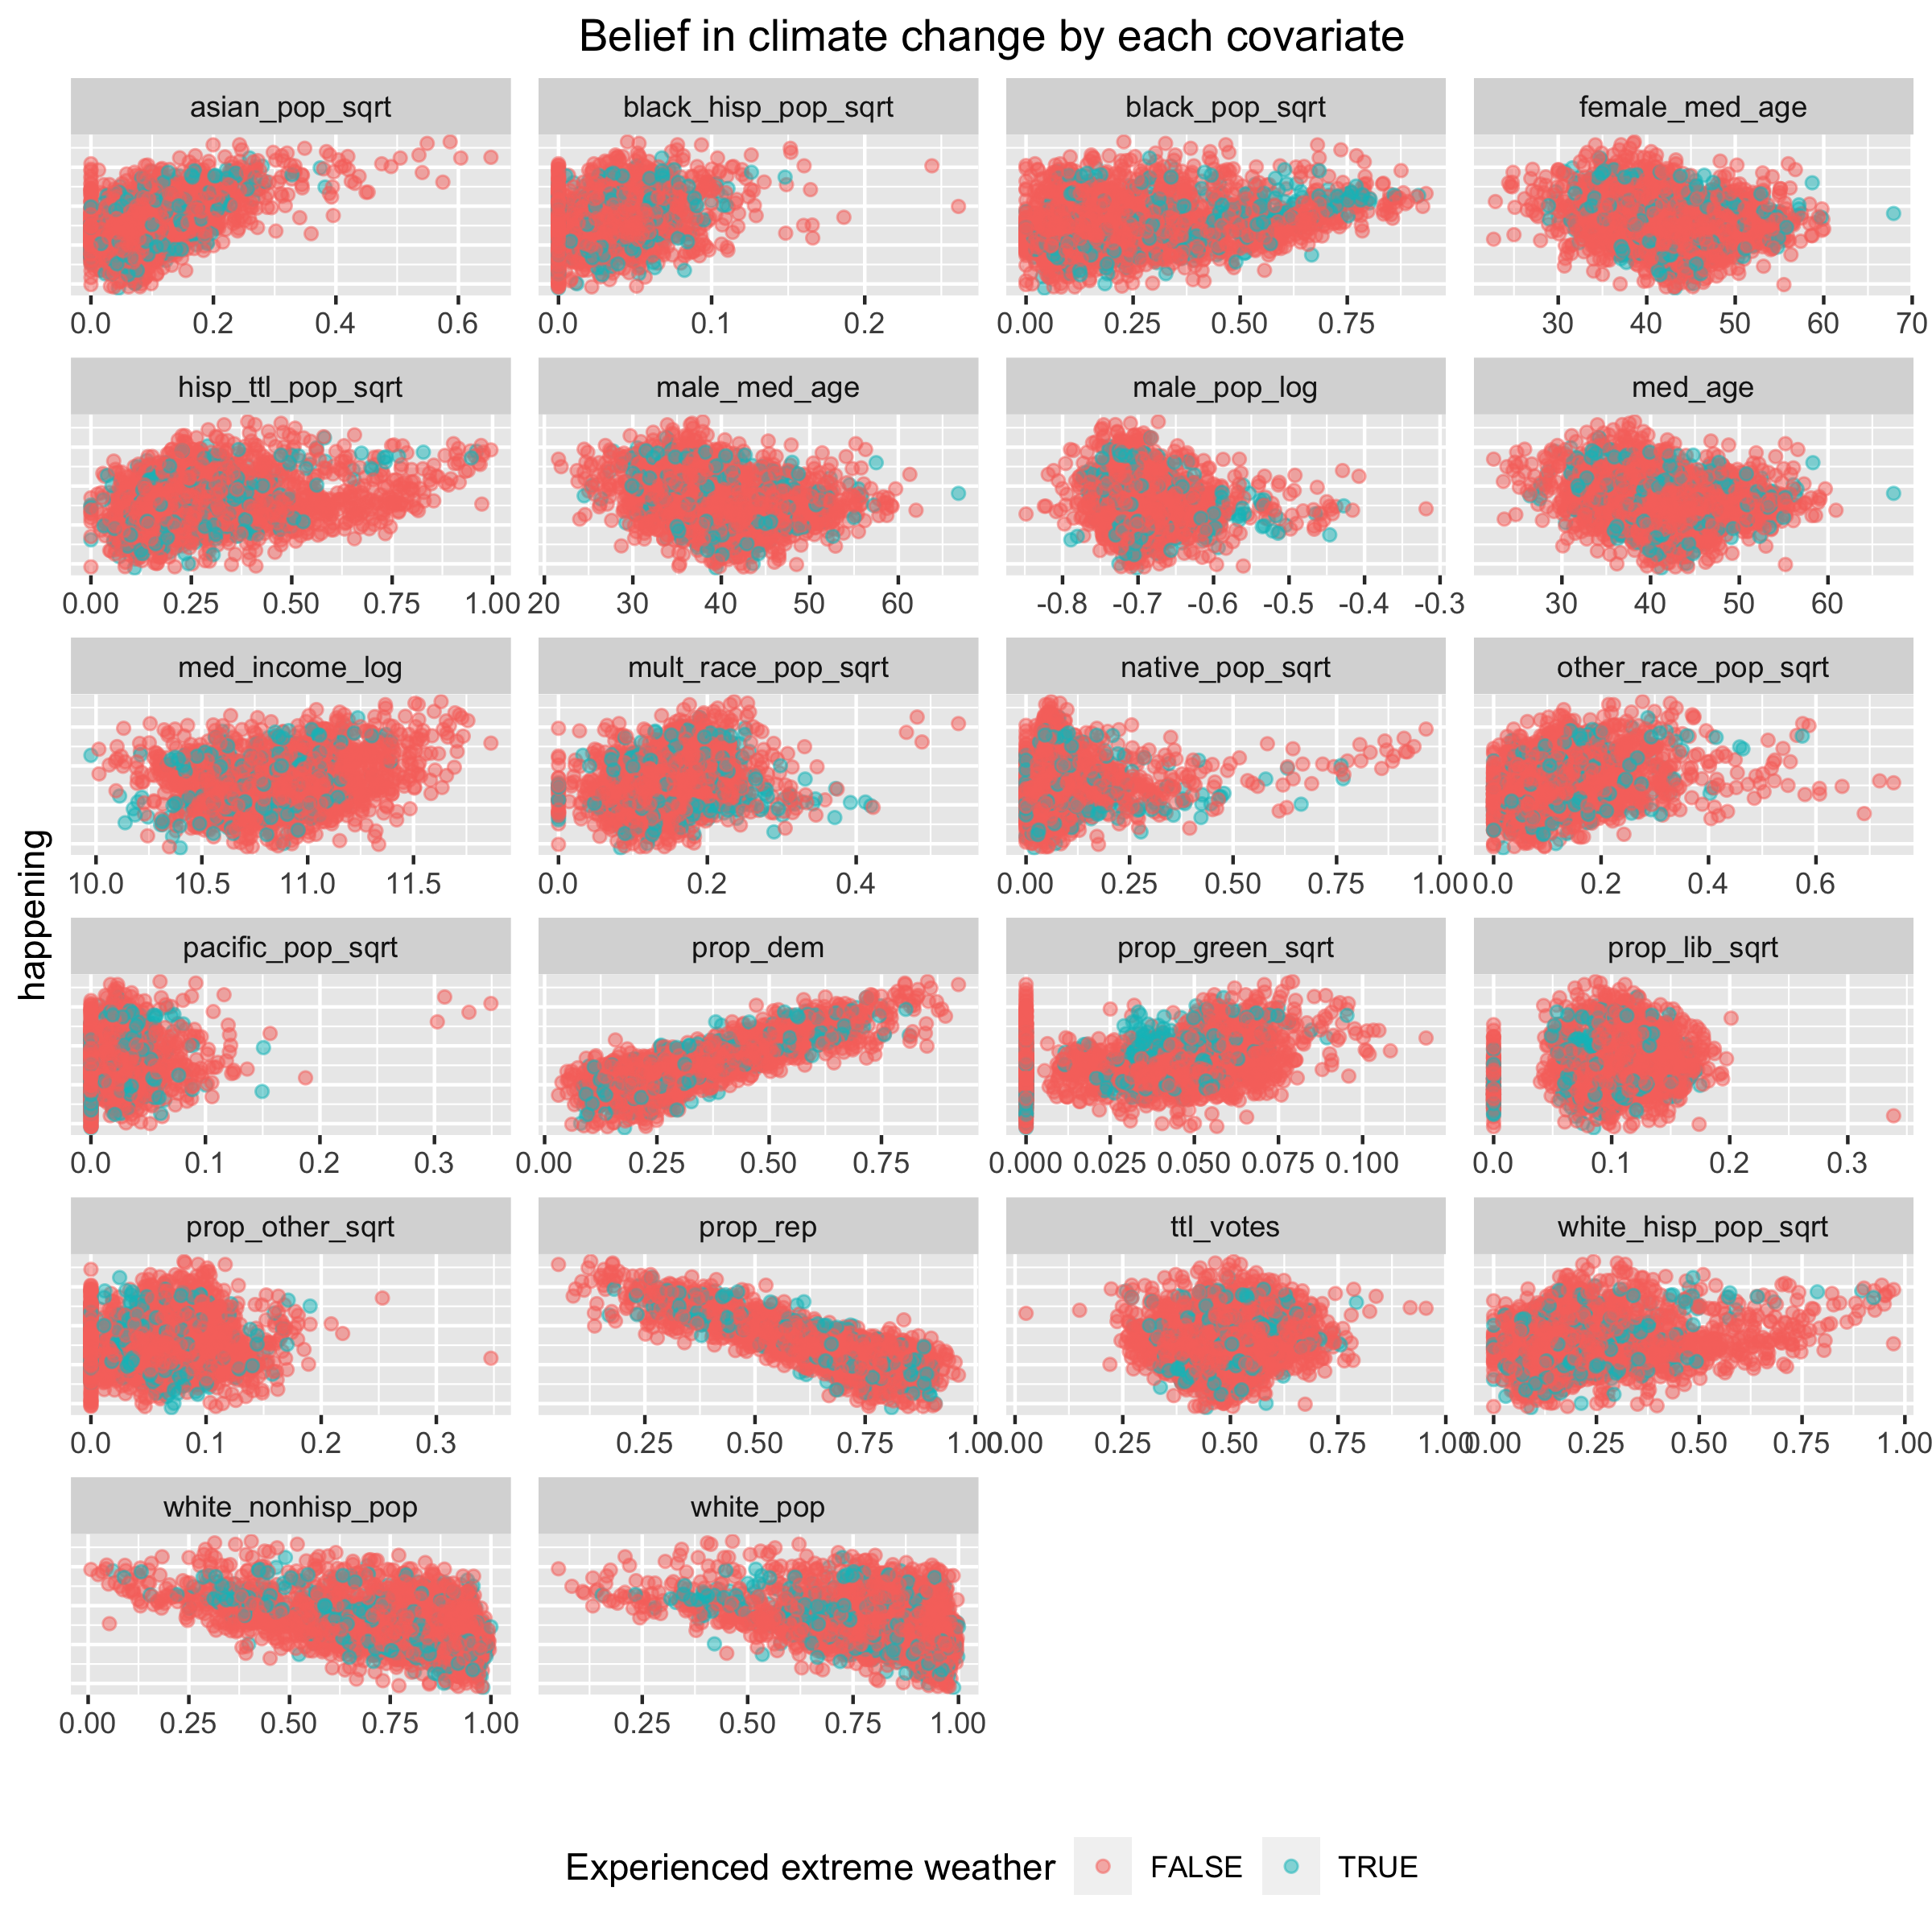
\includegraphics[scale=0.2]{images/covariates_vs_happening.png}
\caption{All covariates are plotted with the response variable `happening' to verify that relationships appear to be roughly linear. If variables have been transformed, their titles end in ``sqrt" or ``log" to represent the appropriate transformation.}
\end{figure}

Before performing Lasso, a few variables that were strongly correlated with other covariates were dropped from consideration: the proportion of county vote towards the Republican party (which is almost perfectly negatively correlated with vote towards the Democratic party), and median age for the male and female populations (which is almost perfectly correlated with the aggregate median age). After normalizing the data, the glmnet R package was used to tune for $\lambda$ using cross validation on a training set of randomly selected counties. Using the resulting "best" tuning parameter, Lasso regression was then run again over both the training and test data. The resulting coefficients are shown in the appendix, ordered by descending absolute value. 

The clearest result of the Lasso procedure was that proportion of votes towards Democrats/Republicans was by far the largest coefficient, indicating the strength of political leaning as a predictor of climate change beliefs. Intuitively, this is not surprising. To see just how much political leaning alone could explain about the variance of climate change beliefs, a simple one-way ANOVA test was performed on average belief in climate change between counties that voted majority Democrat and counties that voted majority Republican. The test is visualized in the boxplot below, the resulting p-value of $<0.01$ strongly rejecting the null that political affiliation has no impact on climate change belief.

\begin{figure}[H]
\centering
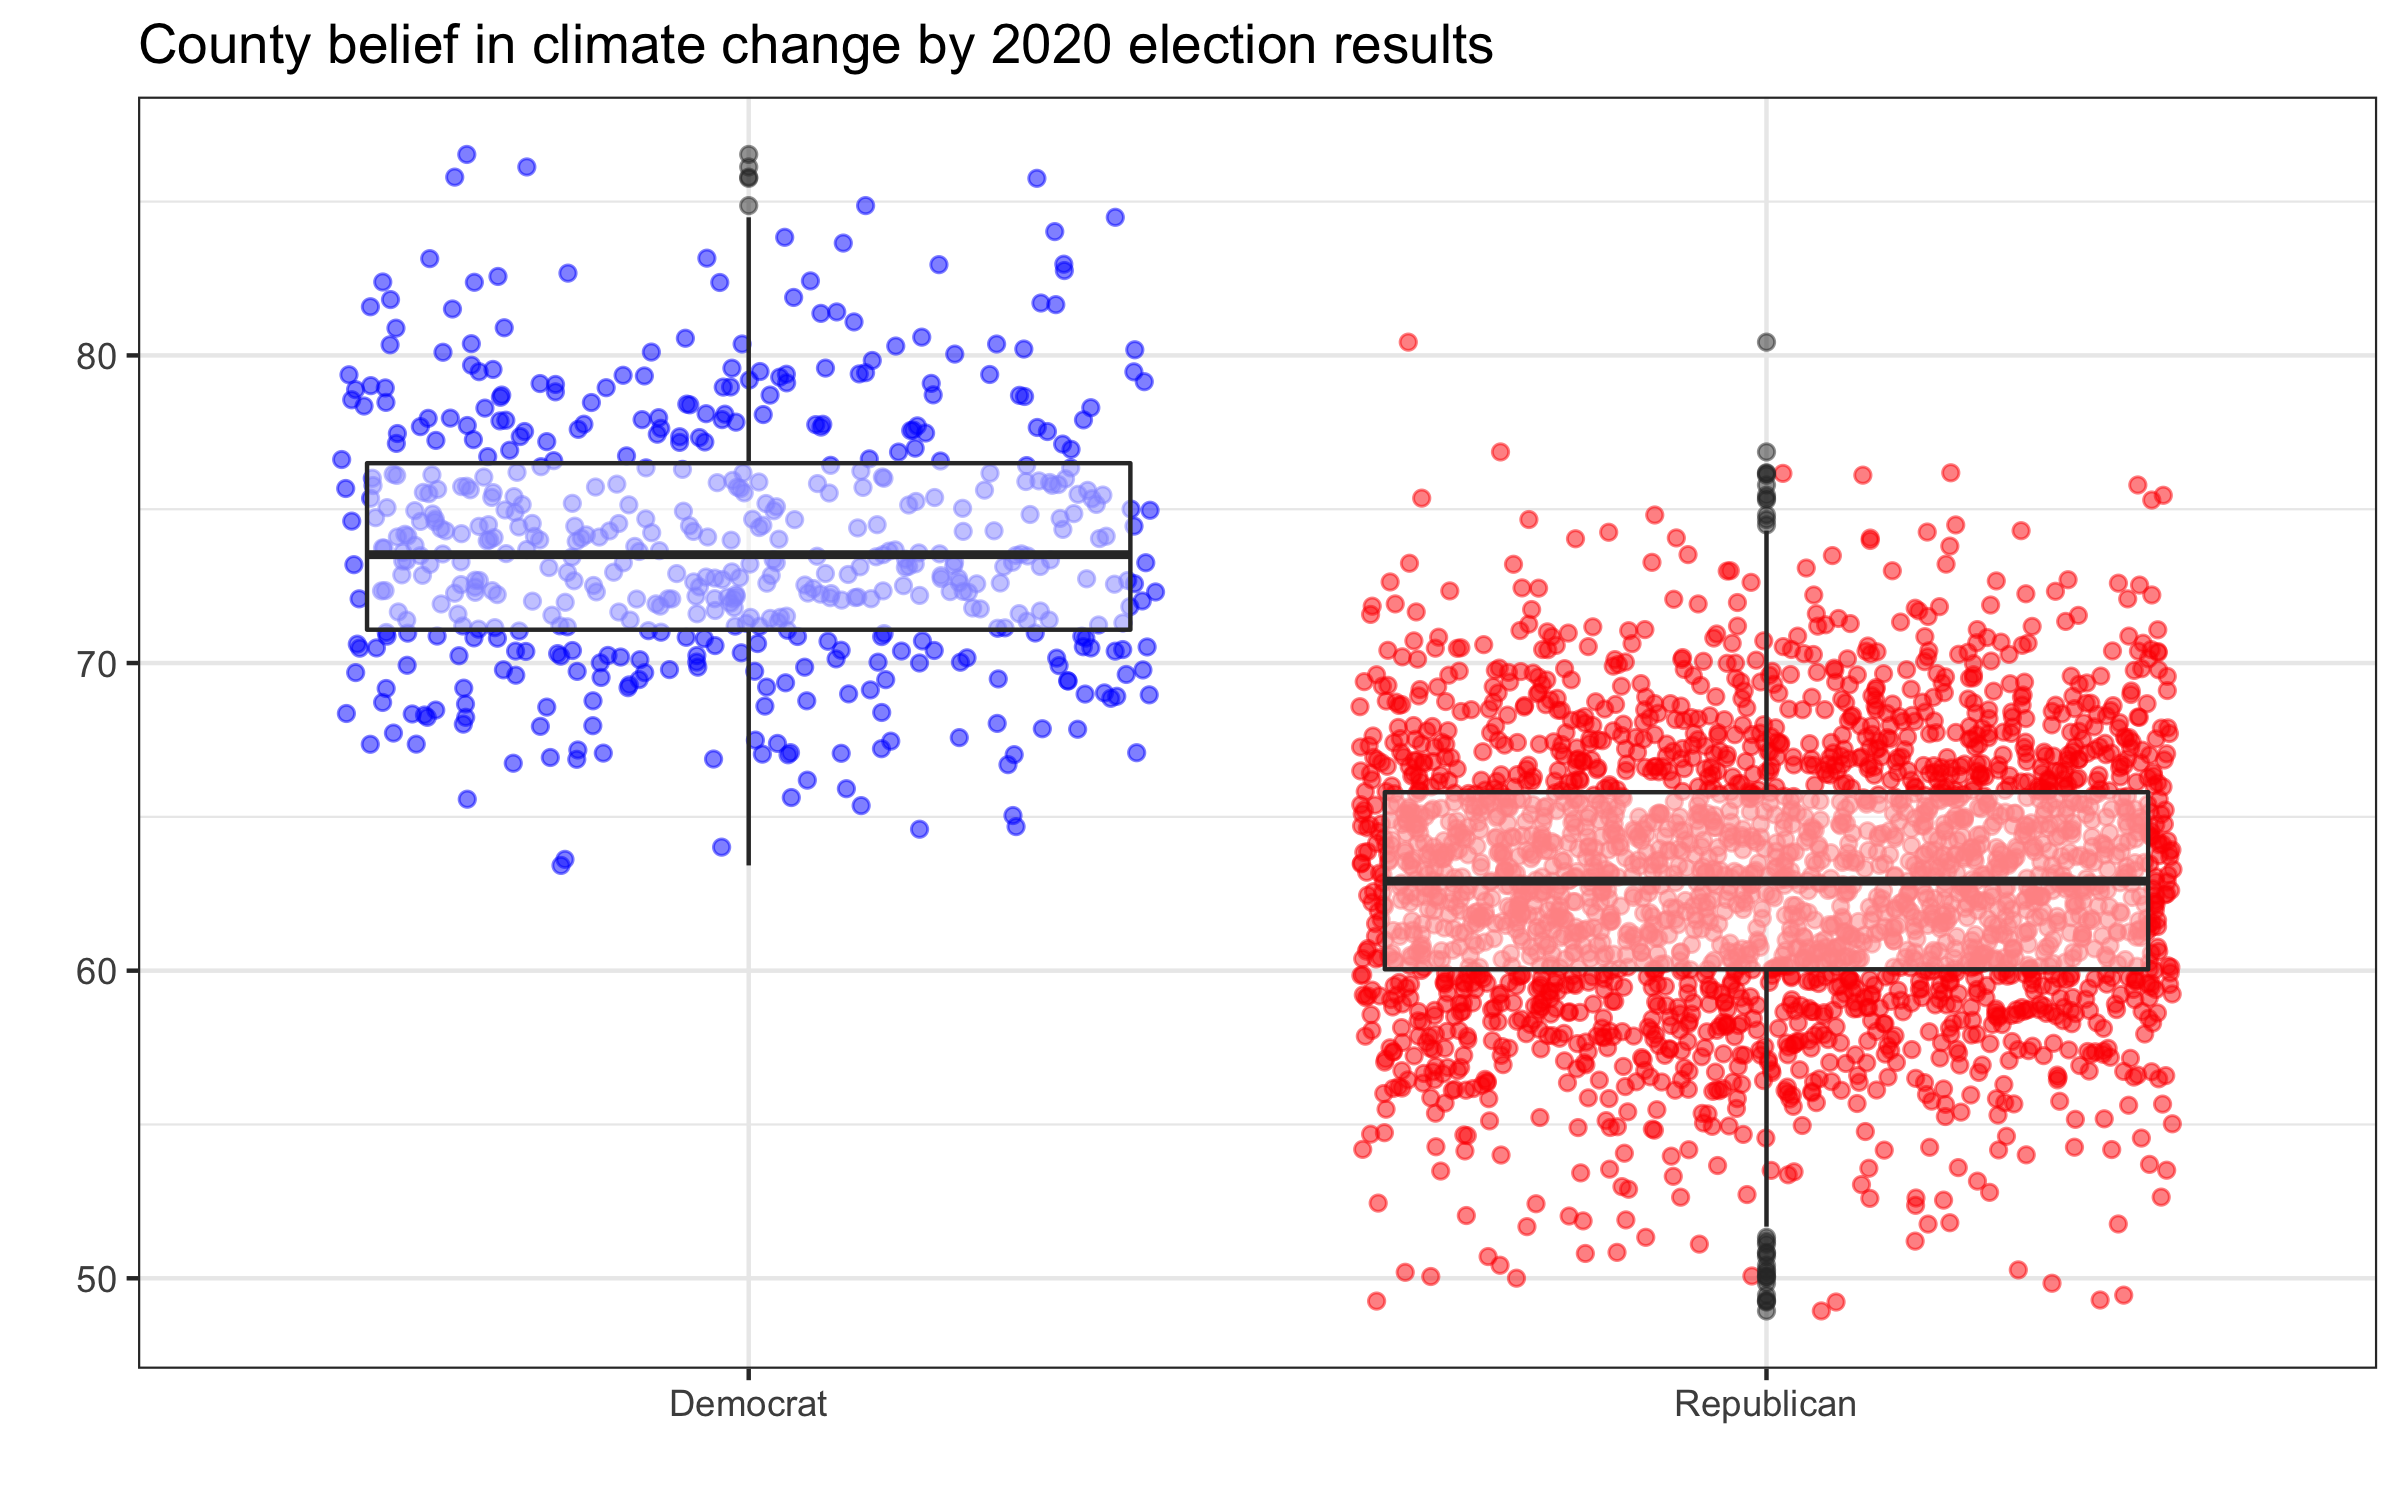
\includegraphics[scale=0.2]{images/election_party_anova.png}
\caption{On average, counties that voted majority Democrat in the 2020 general election are estimated to have about 74\% of county population believing in climate change, while counties that voted majority Republican are estimated to have about 63\% of county population believing in climate change. This is a difference of 11\%, and the resulting t-statistic is -54.21.}
\end{figure}

Note that the data met the requirements for ANOVA testing. The distribution of climate change beliefs is approximately Normal (this is shown in the appendix), these responses are assumed to be independent, and the variance between groups is approximately equal (the standard deviation of the response for Republican-leaning counties is approximately 4.32, while the standard deviation of the response for Democratic-leaning counties is approximately 4.12). 

\subsection{Exploratory clustering}
A manual clustering approach was applied to the data at this point to see how counties similar to each other in higher level terms compared with respect to climate change belief. Unsupervised clustering could also have revealed interesting relationships, but the purpose at this point was to explore interpretable relationships between covariates, the response, and extreme weather, to inform further analysis. To minimize the number of clusters, five of the covariates weighted with the largest magnitude coefficients in the Lasso procedure discussed above were used to differentiate counties at this point: political leaning, total Hispanic population proportion, non-Hispanic white population proportion, proportion of population that voted in 2020, and the proportion of libertarian vote. Each variable was manually discretized into two categories each. Political leaning was split by which party won the majority of each county's vote. Population proportion thresholds were determined using the national proportion of that group in 2019, and then used to bucket counties into "high" or "low" categories. The mean voter turnout value across counties happened to be around 50\%, making that a convenient and sensible threshold. Finally, the proportion of libertarian vote was determined also by comparison to the mean proportion across counties. The resulting 32 clusters were then split further into pairs based on whether or not they had experienced extreme weather.

To maintain the ANOVA assumption of equal variances, pairs were removed from the cluster analysis if the maximum standard deviation of the pair exceeded the minimum standard deviation by 2 or more. Pairs were also removed if one or both clusters had less than 20 counties attributed to it. Only five pairs of clusters survived these requirements, and Q-Q plots were checked for each of these clusters to ensure that the responses of each were roughly Normal. Finally, ANOVA was performed on each pair, testing the null hypothesis that the mean climate change belief of each cluster (differing only by the experience of extreme weather) was the same. To account for multiple testing, the Benjamini-Hochberg correction was applied to control for false detection rate. This less conservative test controlling the FDR was used rather than a correction such as Bonferroni because stakes are low if there is a false positive, so it seems appropriate rather than controlling for family-wise error.

Only one pair resulted in a significant result (to the $\alpha = 0.05$ level): for counties that were Republican leaning, above-average white and below-average Hispanic, with high voter turnout and low libertarian vote, the test found that experiencing a weather event had a small, positive effect on climate change beliefs. The lack of other insights here, partly because many clusters could not be tested due to small sample sizes, motivates the following matching and regression approaches.

\begin{center}
\begin{table}
\begin{tabular}{| c | c | c | c | c | c | c | c | c | c | c ||}
\hline
Pair & Political & Hisp. Pop. & White Pop. & Voter Turnout & Libert. Vote & $n$ & Mean Diff. & p-value & BH p-value \\ [0.5ex]
\hline
\hline
1 & Red & Low & High & High & Low & 397, 104 & 1.2466 & 0.0052 & 0.0260 \\
\hline
2 & Red & Low & High & Low & Low & 423, 130 & -0.1445 & 0.7159 & 0.9775 \\
\hline
3 & Red & Low & Low & Low & Low & 71, 26 & 0.2999 & 0.6399 & 0.9775 \\
\hline
4 & Red & Low & High & High & High & 572, 57 & -0.0151 & 0.9775 & 0.9775 \\
\hline
5 & Red & Low & High & Low & High & 360, 68 & -0.4512 & 0.3794 & 0.9775 \\
\hline
\end{tabular}
\caption{Results of clustering analysis. Values for $n$ are listed in the order: did not experience extreme weather, did experience extreme weather. Positive mean difference values indicate that counties that did experience extreme weather had higher average belief in climate change than those those that did not.}
\end{table}
\end{center}


\subsection{Matching}
The lack of satisfying results from the exploratory clustering approach helps to motivate a different tactic: individually matching similar counties that differ on their extreme weather experience. To accomplish this, the R package MatchIt was used. This package is developed for causal inference applications, and "performs pairing, subset selection, and subclassification with the aim of creating treatment and control groups balanced on included covariates", as stated in its documentation. This analysis does not consist of a proper causal inference framework, for reasons including the lack of randomization between "treatment" of experiencing an extreme weather event, and the fact that belief estimates are obtained only at the county level rather than the individual level. However, the package and ideas behind comparing "treatment" and "control" group responses are still helpful for the goals of this report. Using MatchIt, counties that were flagged as experiencing extreme weather were matched to counties that did not, but were as similar as possible to the first county with respect to the selected covariates, which are unchanged from the Lasso-identified coefficients used in the clustering exercise. In particular, the "optimal" matching method option was used, which minimizes the sum of absolute pairwise distances in the matched sample. This lowers the probability of extreme within-pair distances with respect to covariates. Figure 6 shows the effects of matching on the standardized mean difference of the covariates of counties with and without the extreme weather flag. Note that the matching process resulted in 511 pairs, with no two control counties matched to the same extreme weather county.

\begin{figure}[H]
\centering
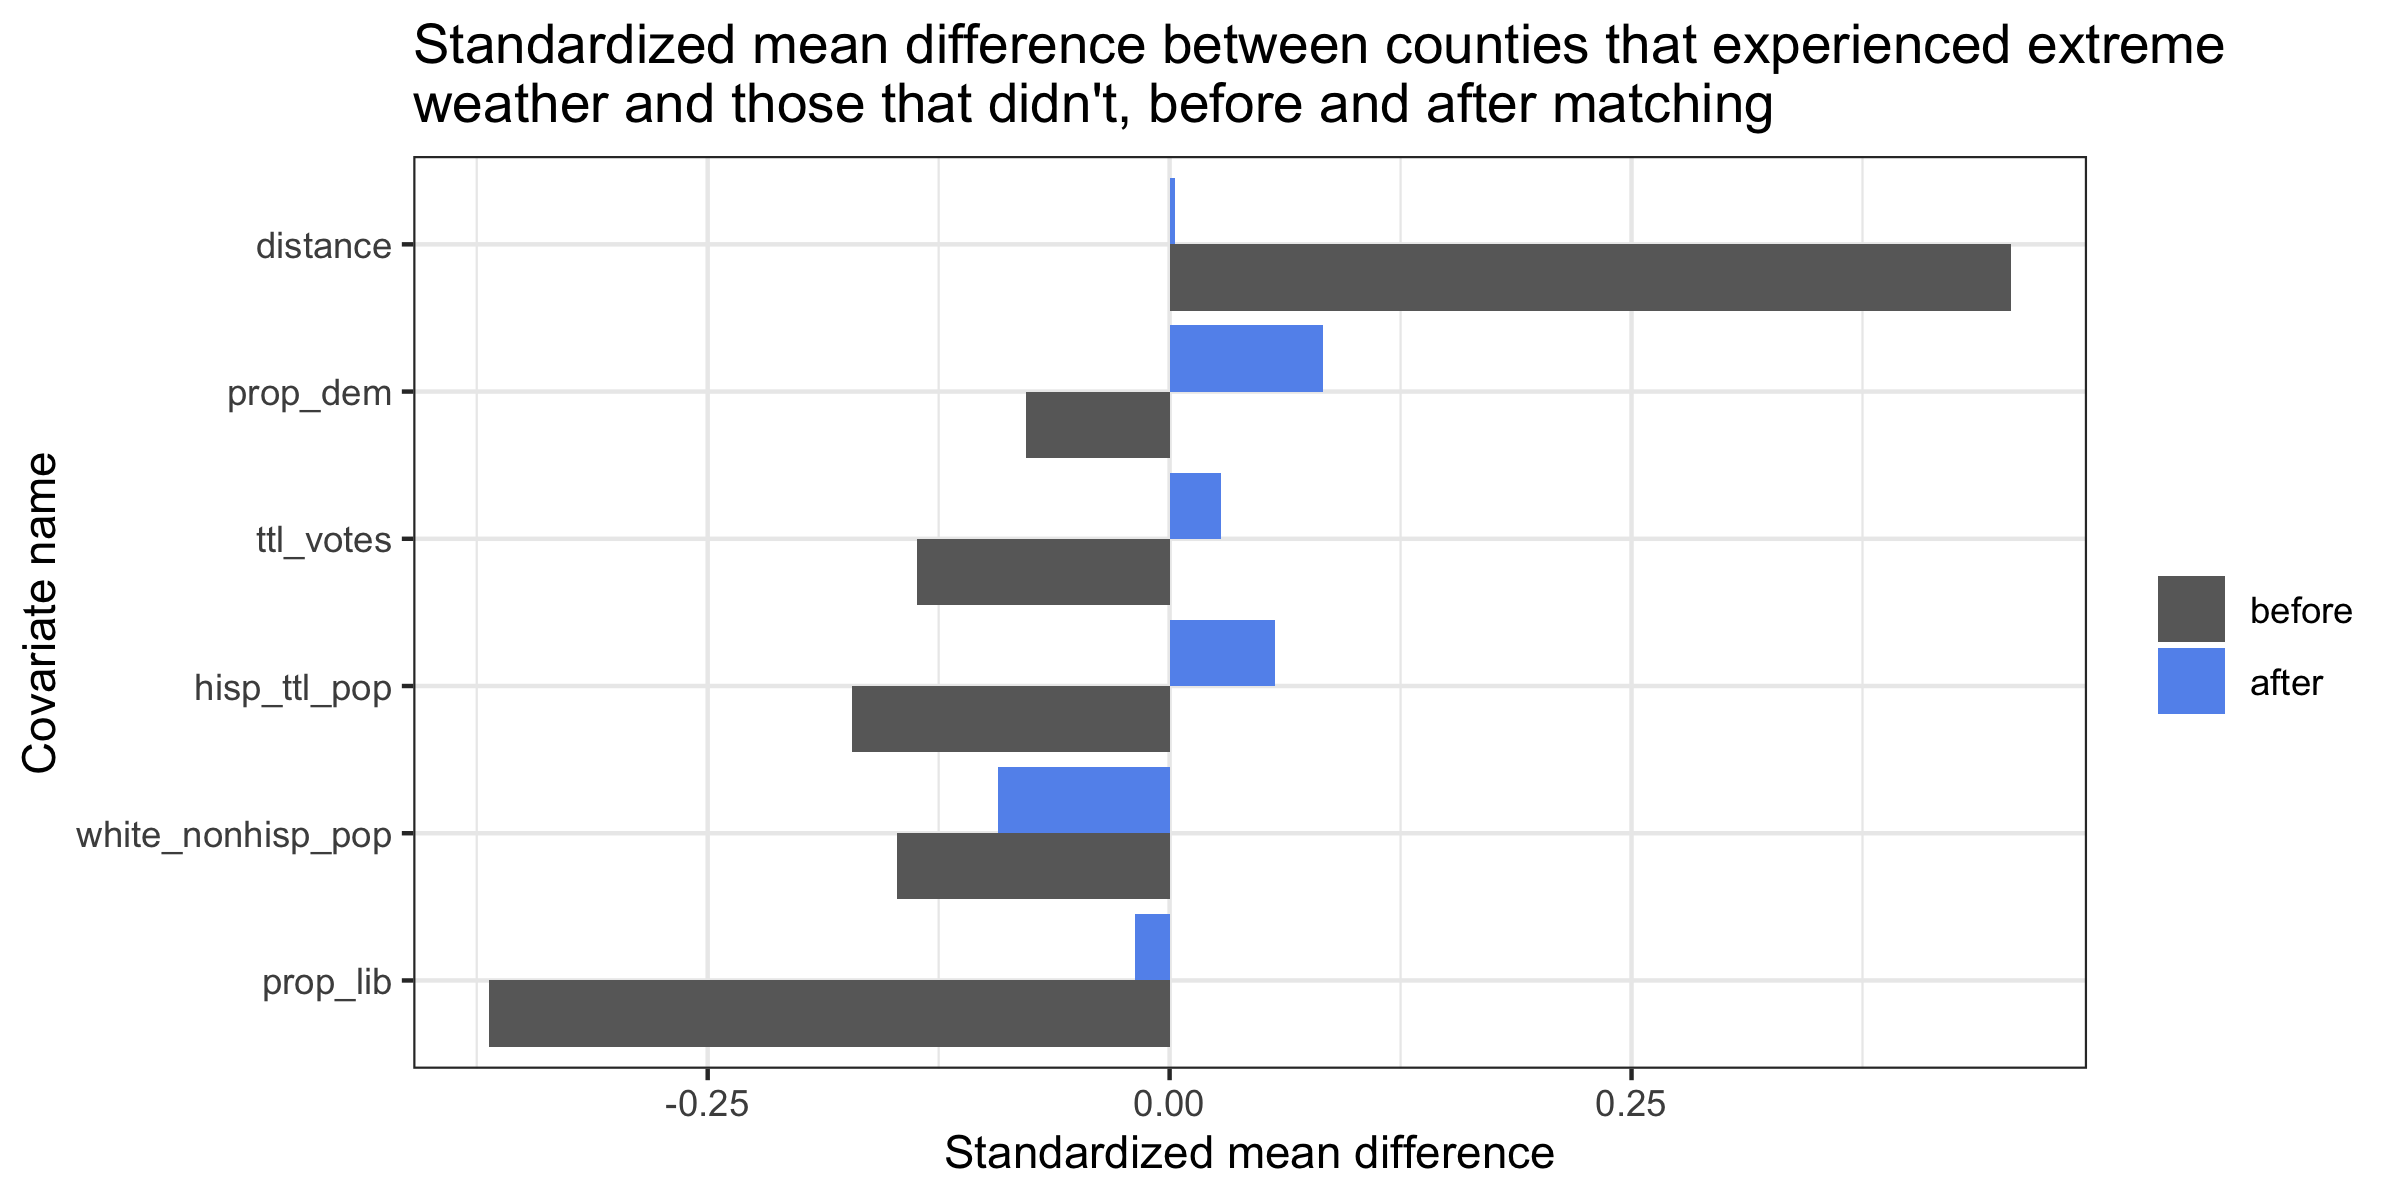
\includegraphics[scale = 0.2]{images/matching_balance_plot.png}
\caption{This figure shows that matching via MatchIt was able to improve the standardized mean difference between almost all covariates, though the Democrat proportion of votes remains virtually unchanged in magnitude but changes sign.}
\end{figure}

Once counties were matched, a paired t-test was performed to test the null hypothesis that the mean difference in climate change belief between pairs was zero. The results are reported in the Results section below, and a Q-Q plot is included in the appendix to demonstrate that Normality assumptions were met. 

\subsection{Regression}
Linear regression was used to get a second opinion on the relationship between extreme weather experience and climate change belief, holding other covariates constant, but also to get an overall picture for how all covariates contribute to climate change belief. In the matching procedure, the number of covariates was limited to try to allow for closer pairwise matches between the most predictive (as determined by Lasso) variables. This constraint doesn't need to apply to the regression model, so more covariates were included among those given larger coefficients by Lasso (though some were still omitted to avoid collinearity from inclusion of too many dependent proportions). 

Model diagnostic tests passed for the resulting model, as the residuals appeared to be close to Normal and residual variance looked fairly equal across fitted values. Plots demonstrating these tests can be found in the appendix, and the regression summary is included in the results section. 

\section{Results}
\subsection{Matching}
The paired t-test performed on matched counties found that the mean difference in climate change opinion of 0.7464 was significant to the $\alpha = 0.05$ level, rejecting the null hypothesis that the mean difference is 0. The table below summarizes these results.

\begin{table}[H]
\centering
\begin{tabular}{|| c | c | c | c ||}
\hline
n & mean difference & t & p-value \\ [0.5ex]
\hline
\hline
511 & 0.74641 & 2.1875 & 0.02916 \\
\hline
\end{tabular}
\caption{Results of paired t-test, methods described in Matching subsection of Analysis.}
\end{table}

Though this paired t-test is not testing whether the nonzero mean difference is truly positive or negative, only if it is nonzero, the metric value does imply that experiencing extreme weather corresponds to a small increase in climate change belief.

\subsection{Regression}
The summary of the linear regression analysis is displayed in Figure 7, where we can see that the coefficient of the flag for witnessing extreme weather is small, positive, and significant to the $\alpha = 0.001$ level. This value indicates that counties that witnessed an extreme weather event are likely to have a slightly higher belief in climate change by about 0.48 (in percentage, not proportion). As expected, counties with a higher proportion of the 2020 election vote going to Joe Biden are much more likely to believe in climate change, and to a lesser extent, so are counties with a higher proportion of the vote to the libertarian candidate. Interestingly, counties with an older median age are predicted to also be slightly more likely to believe in climate change, which may be surprising as a common perception is that younger generations care much more about the environment. Proportions of different race and ethnicity groups seem to have some different relationships with climate change belief: counties with a larger non-Hispanic, white population or larger Black population are predicted to be less likely to believe in climate change, while counties with a larger Asian or Hispanic population are predicted to be more likely to believe in climate change. The voter turnout also has a significant coefficient in this model, indicating that counties with higher voter turnout rates in the 2020 general election tend to also have stronger beliefs in climate change.

\begin{figure}[H]
\centering
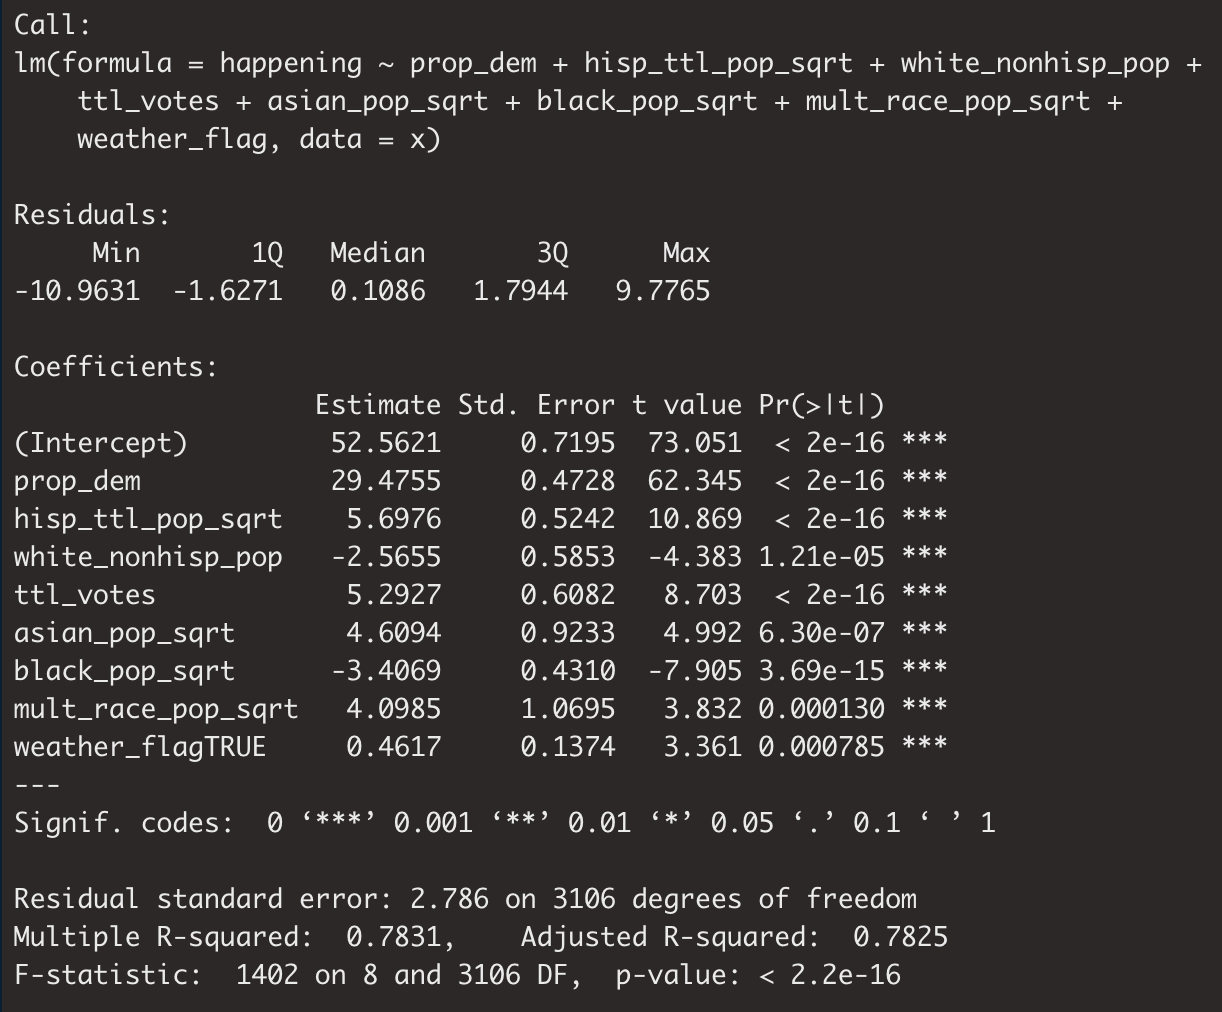
\includegraphics[scale=0.5]{images/regression_summary.png}
\caption{Summary of linear regression model predicting county climate change belief.}
\end{figure}


\section{Conclusion}
The results of the multiple approaches explored in this analysis imply that recently experiencing an extreme weather event, in places where these types of events have become more common over the past 5 years, may increase the likelihood of the average individual believing that climate change exists. The matching and linear regression approaches agree on this point. However, these effects may be heterogeneous between subsets of the population with different racial, socioeconomic, and political features, though this analysis is limited in its exploration of differences between such subsets via the cluster analysis described here. As one may expect, the linear regression approach and a simple ANOVA test demonstrated how strongly political leaning influences climate change belief, indicating that even if more convincing effects of extreme weather were found, they would still likely be eclipsed by the effect of political polarization. 

\newpage
\section{References}

\subsection{Contextualizing the problem of climate change and climate change communication}
\begin{itemize}
	\item Guardian article about current climate change crisis: \url{https://www.theguardian.com/environment/ng-interactive/2021/oct/14/climate-change-happening-now-stats-graphs-maps-cop26}
	\item Organization for climate change communication: \url{https://climate-xchange.org/communicating-the-climate-crisis/}
	\item Yale Climate Communication Group: \url{https://climatecommunication.yale.edu/}
\end{itemize}

\subsection{Data sources}
\begin{itemize}
	\item Climate change opinion data: \url{https://climatecommunication.yale.edu/visualizations-data/ycom-us/}
	\item Election data: MIT Election Data and Science Lab, 2018, "County Presidential Election Returns 2000-2020", \url{https://doi.org/10.7910/DVN/VOQCHQ}, Harvard Dataverse, V9, UNF:6:qSwUYo7FKxI6vd/3Xev2Ng== [fileUNF]
	\item Census Bureau ACS Estimates: \url{https://www.census.gov/programs-surveys/acs/data.html}
	\item FEMA disaster data: \url{https://www.fema.gov/about/openfema/data-sets#disaster}
\end{itemize}

\subsection{Analysis documentation}
\begin{itemize}
	\item MatchIt package: \url{https://kosukeimai.github.io/MatchIt/reference/method_optimal.html}
	\item TidyCensus package: \url{https://cran.r-project.org/web/packages/tidycensus/tidycensus.pdf}
\end{itemize}

\newpage
\section{Appendix}

\begin{figure}[H]
\centering
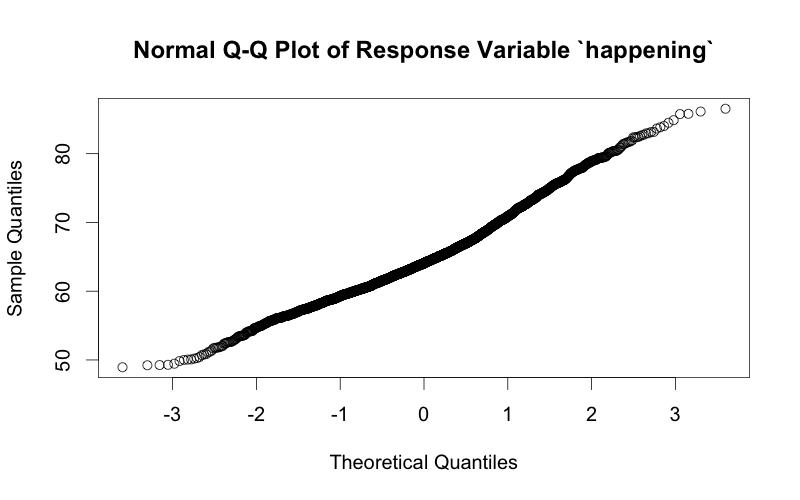
\includegraphics[scale=0.5]{images/response_qqplot.png}
\caption{The response variable, the estimated proportion of county population that believes in climate change, is approximately Normally distributed.}
\end{figure}

\begin{figure}[H]
\centering
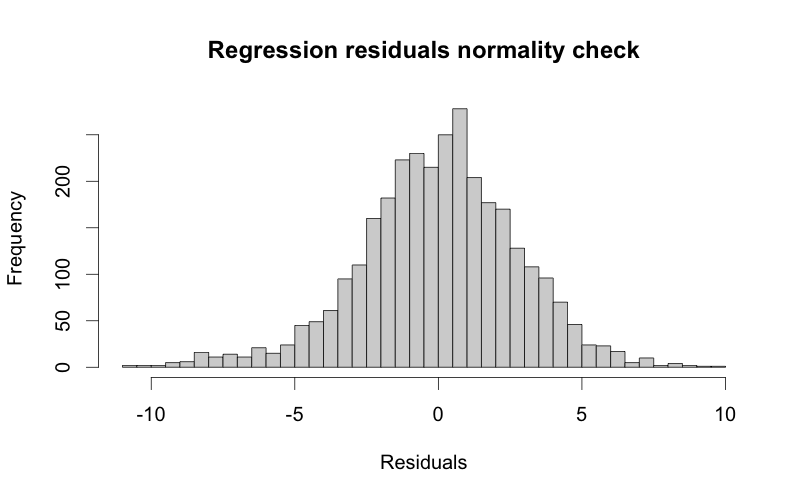
\includegraphics[scale=0.5]{images/regression_residuals_hist.png}
\caption{Histogram of the residuals from the linear model discussed in the analysis section.}
\end{figure}

\begin{figure}[H]
\centering
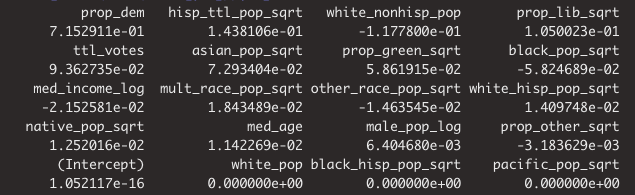
\includegraphics[scale=0.5]{images/lasso_train.png}
\caption{Coefficients resulting from Lasso regression on the {\bf{training}} data (all covariates that were not extremely correlated included, with training data comprising 50\% of the original counties).}
\end{figure}

\begin{figure}[H]
\centering
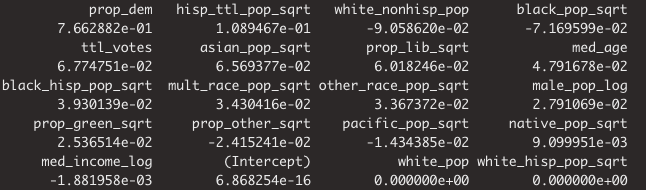
\includegraphics[scale=0.5]{images/lasso_test.png}
\caption{Coefficients resulting from Lasso regression on the {\bf{test}} data (all covariates that were not extremely correlated included, with training data comprising 50\% of the original counties).}
\end{figure}

\begin{figure}[H]
\centering
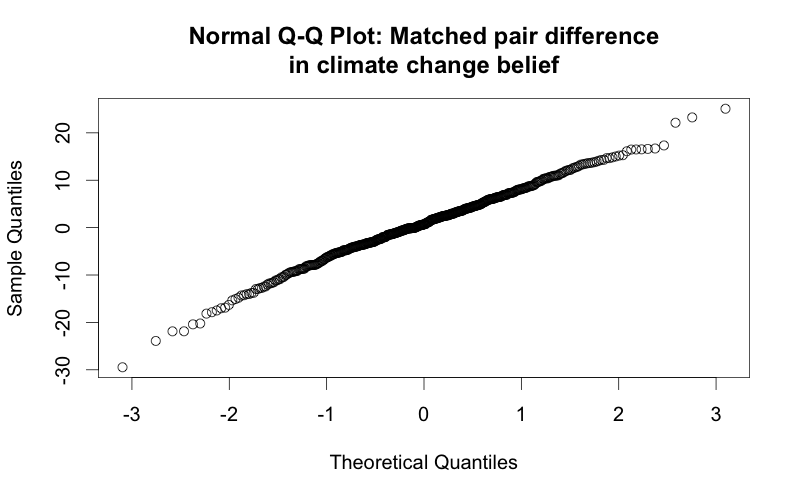
\includegraphics[scale=0.5]{images/matched_pair_qq.png}
\caption{Normality check for the differences in climate change belief among matched pairs described in the Matching section.}
\end{figure}

\begin{figure}[H]
\centering
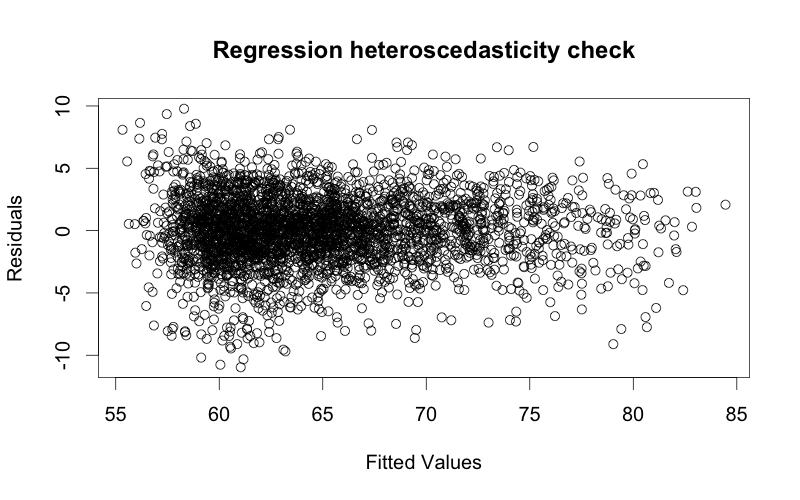
\includegraphics[scale=0.5]{images/regression_variance_check.png}
\caption{Heteroscedasticity model diagnostic plot for the linear model discussed in the analysis section.}
\end{figure}



\end{document}